% ------------------------------------------------------------------------------
% A primer on continuum models and how this relates to the work we have done
% 1) Introduce logistic growth and diffusion
% 2) Introduce FKPP in all its glory .
% 3) Show one and two d spread
% 4) Couple to the sub-grid, what this says about the sub-grid...
% 5) Talk about growth rate-alpha and growth rate of sub-grid... an assumption about mixing and SIR <--         appendix territory
% 6) Show `toy model properties in alpha and d' get realistic looking spread...
% 7) Show realistic spread and give a primer to things which could be done.
% 8) Talk about alternate more, non-linear models and consult Rammile...
% ------------------------------------------------------------------------------

\chapter{Continuum Models of tree diseases}
The typical approach is spatial-$SIR$ \textcolor{red}{REVIEW SPATIAL SIR}, however, tree disease is localised and will does not fit well to an $SIR$ model\textcolor{blue}{CITE MASTERS PROJECT (unpublished)}. %whose  Masters project is this ??
As such we opt for 

\textcolor{blue}{Lit-review: 1) PDE/continuum models for disease 2) reaction-diffusion models}
\textcolor{red}{This chapter takes a different modelling approach from the ones seen so far. %
A continuum approach, formulated on reaction diffusion equations, is used to describe the spread of disease. %
The aim of this Chapter is to offer a first approximation towards a continuum model. %
PDE models have been  studied rigorously in the context of biological waves, disease and population dynamics. %
The most basic reaction diffusion equation is the Fisher equation, also known as the the Kolmogorov–Petrovsky–Piskunov equation or FKPP equation for short. %
FKPP equation. This equation makes for an attractive off-the-shelf model, with known solutions, well-studied behaviour and a simple form involving both logistic growth and diffusion-based propagation.}                                                


\textcolor{red}{Firstly we establish the two components of reaction-diffusion, that being logistic growth and diffusion, in separate models. Then we proceed to show how diffusion coefficients can be informed by the non-local dispersal model and data sets presented in Chapter \ref{chapter:regional-containment1} }. We explored how modelling individual trees within a map covering GB  was computationally infeasible. Another approach that works around this problem is to use a continuum model. Using a continuous model in the form a partial-differential equation permits the averaging-out of previously discrete quantities, such as the number of infected trees or the concentration of the unit of infected  trees.

 Ahybrid modelling approach was developed, both flexible and generalisable, based on a Monte Carlo sub-grid model at resolution 5m and a reactive-diffusive PDE model at resolution 1km. %
 The Monte Carlo sub-grid model uses a non-local compartmental SIR model and is shown to demonstrate travelling wave-like behaviour when ensemble-averaged. %
 The reaction-diffusion system chosen is the FKPP equation, as the simplest model that  demonstrates the propagation of travelling waves and logistic growth of the pathogen. From simple epidemiological input parameters travelling wave-speeds of the sub-grid are pre-determined and mapped to diffusion coefficients informing the FKPP equation. %
 The FKPP then simulates a pathogen spreading over GB. This framework relies on a species abundance distribution. %
 Although efforts are being undertaken to attain high quality abundance data over large distances, at present no such data is publicly available. %
 For this reason we use modelled abundance data of GB tree species. This chapter contributes in  developing resalable large-scale epidemic models based on small scale epidemiological principles. %

\section{PDE modelling for tree disease}
PDE models are useful because they can model averaged, or smoothed, quantities such as the number of infected trees at each point in time and space. Reaction-diffusion (RD) PDE's  have been used extensively for the purpose of epidemic modelling in space and time, \textcolor{red}{see Chapter \ref{chapter:lit-rev}}. The simplest description that can be used to model the spread of a non-static pathogen comes in the form of a reaction-diffusion PDE. That is, the Fisher-Kolmogorov (FKPP) model. The FKPP model has well-studied solutions that exhibit travelling waves. The FKPP model is based on the diffusion and logistic growth of a given quantity or field $u$. %
Together, the growth and diffusion of a quantity give rise to a self-propagating wave that spreads outwards in time and maintains the same shape.\\

\subsection{The FKPP model}

In one spatial dimension, the FKPP model is given by:
\begin{equation}
\label{eq:fkpp-expo}
    \frac{\partial u}{\partial t} = \mathcal{D}\frac{\partial u}{\partial x} + ru(u - 1)
\end{equation}
where $\mathcal{D}$ is a diffusion coefficient measured in units $\mathrm{m^2 t^{-1}}$ and $r$ is a growth constant (or rate) with units $t^{-1}$. %
This model assumes logistic growth and diffusion of the field $u$. In the context of modelling the spread of disease through a population of trees, the field $u$ constitutes the `concentration' of pathogen at a particular point. %
When the pathogen concentration reaches the maximum value of $1.00$ all susceptible tissue is taken as infected. This is an assumption that could lead to an over-estimation of disease  as pathogens are unlikely to infect all susceptible units of trees in a given region \cite{neher1992underestimation}. %
However,  modifications, for example \ref{eq:fkpp-expo} are possible. One example is seen with the inclusion of a carrying capacity $K$\footnote{A carrying capacity could easily be included into the model given in the logistic growth term $(\frac{u}{K} - 1)$ The field $u$ is then interpreted as a raw number of infected. \textcolor{red}{SEE REFERENCE...}}, here , I keep using   the most basic variant.

\begin{figure}
    \centering
    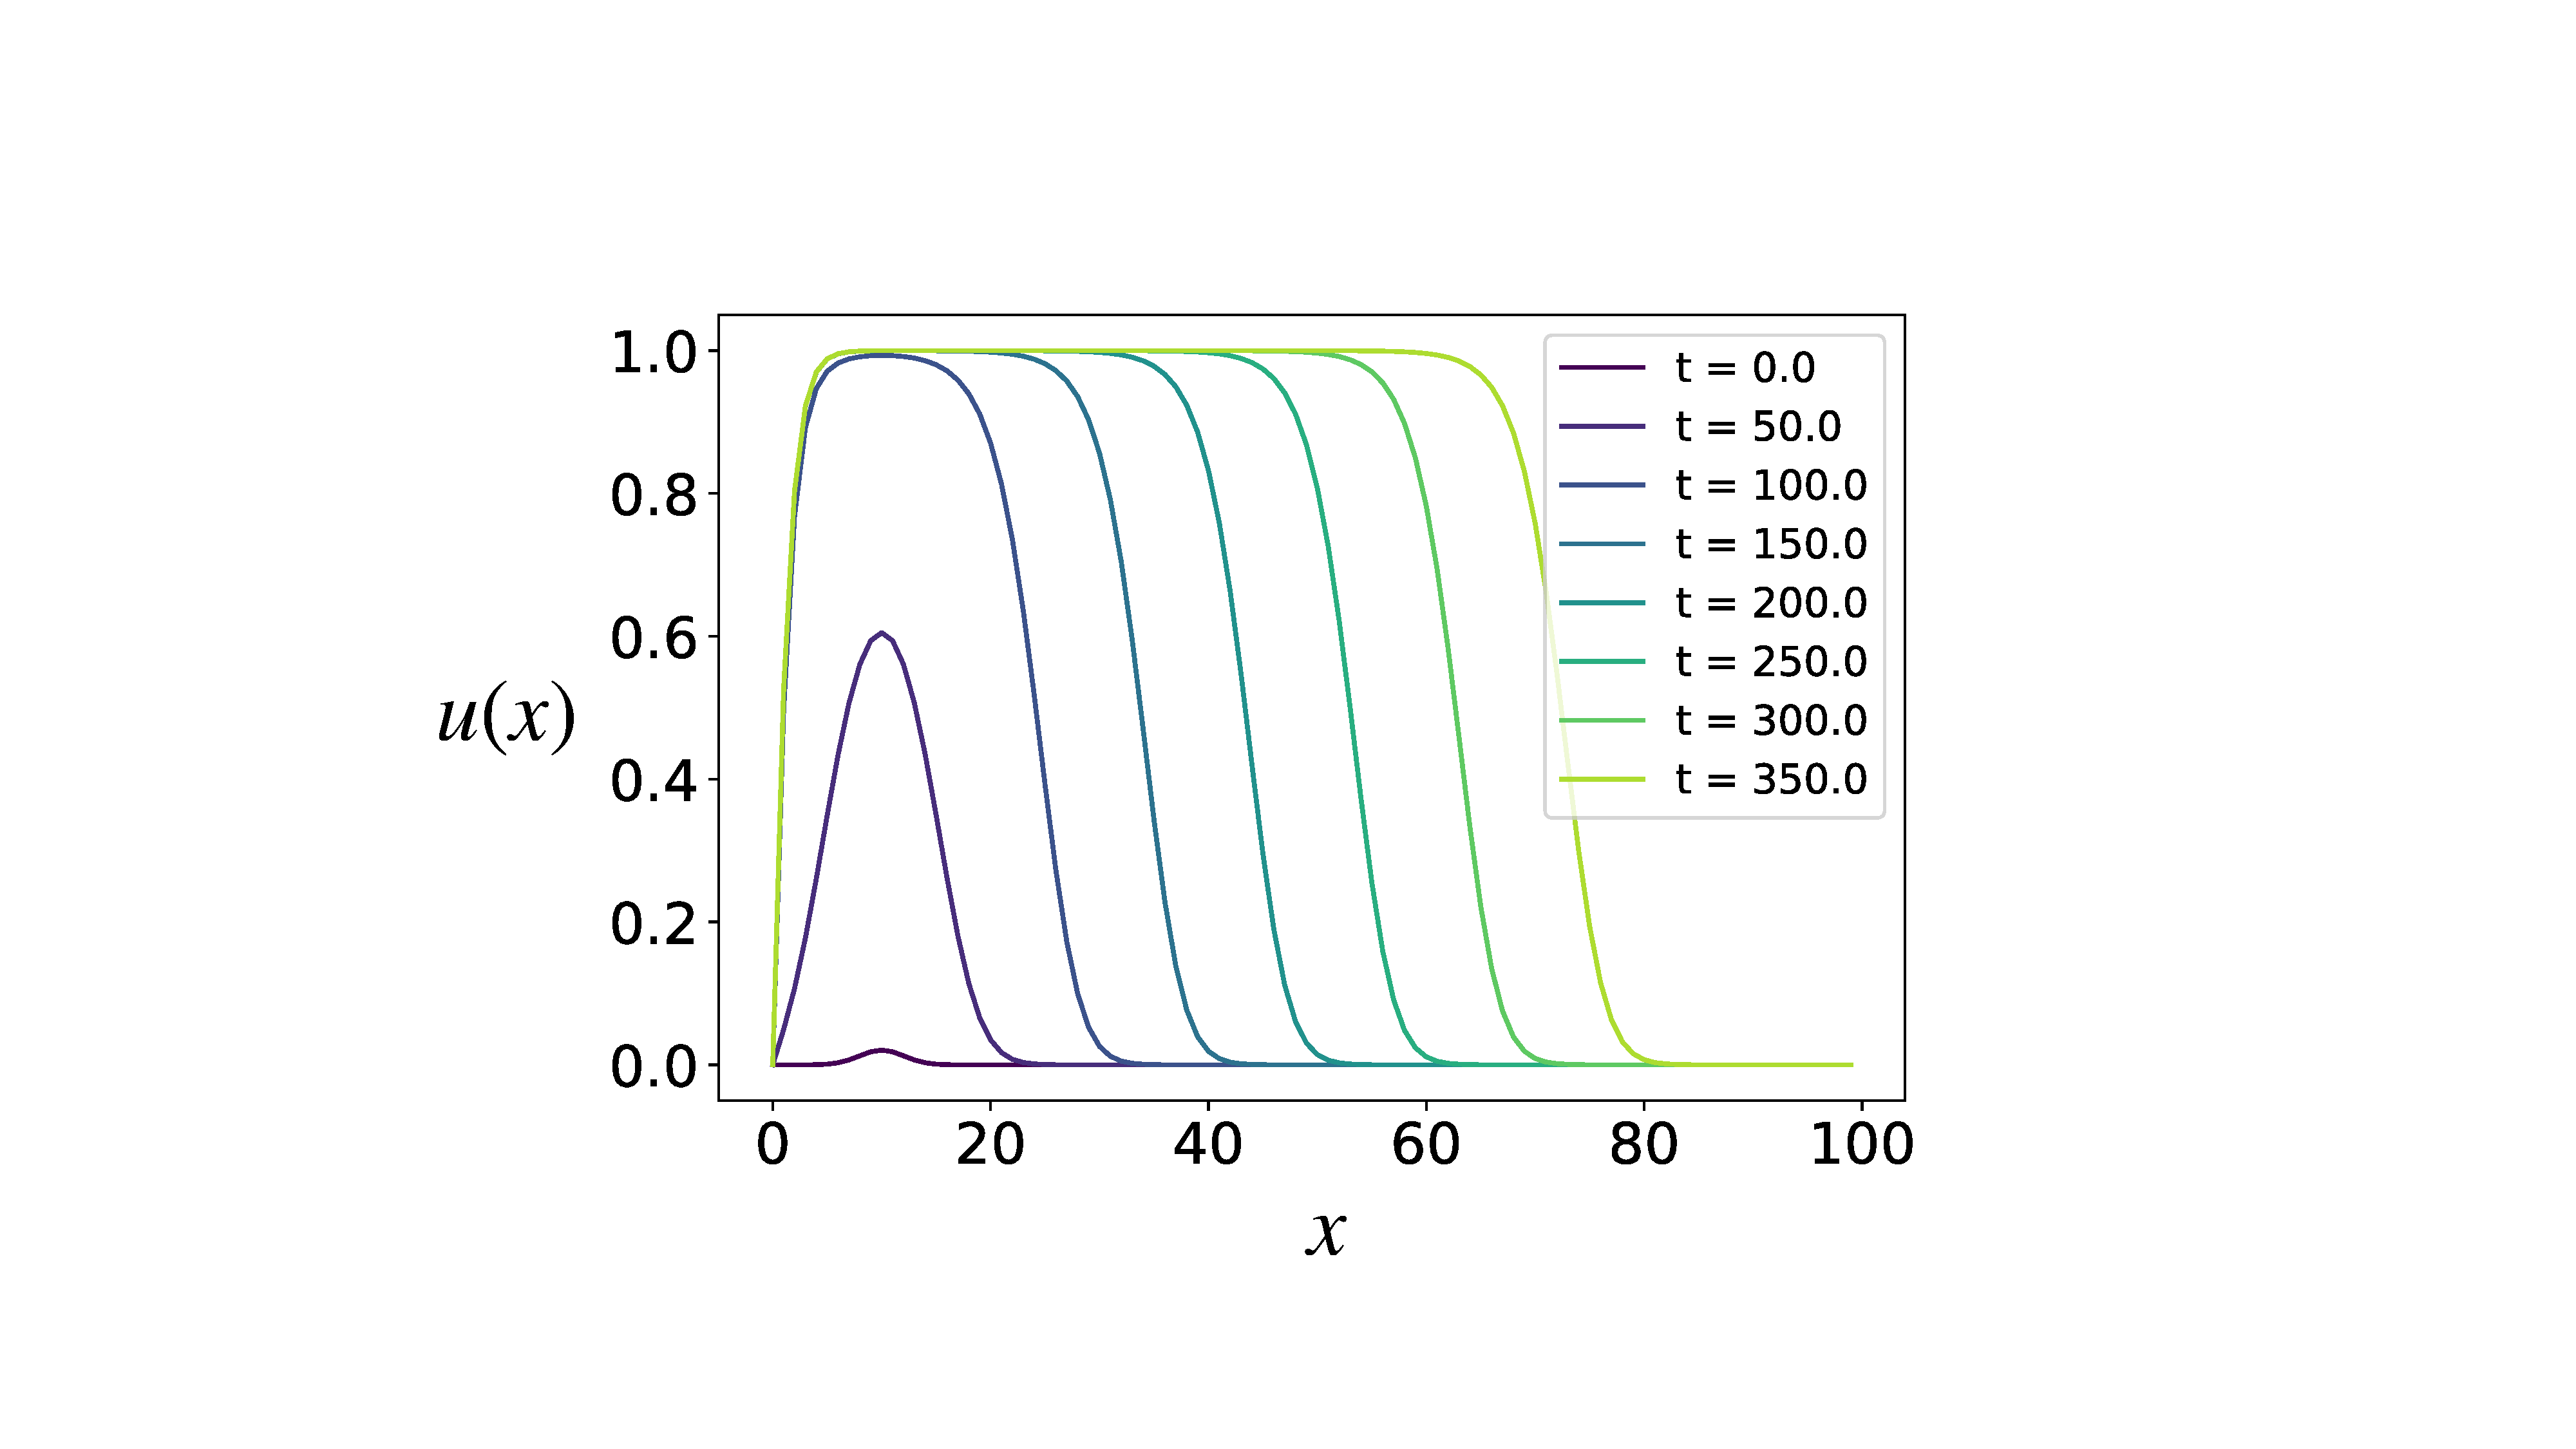
\includegraphics[scale=0.25]{chapter7/figures/figure1xy.pdf}
    \caption{A simulations of the FKPP model for $r=0.10$ and $\mathcal{D}=0.10$ in one spatial dimension. A non-zero field value is initialised at $x=10$ at time $t=0$. Uniform growth and diffusion give rise to a wave-front that propagates with constant speed.}
    \label{fig:fkpp-expo1D}
\end{figure}


\begin{figure}
    \centering
    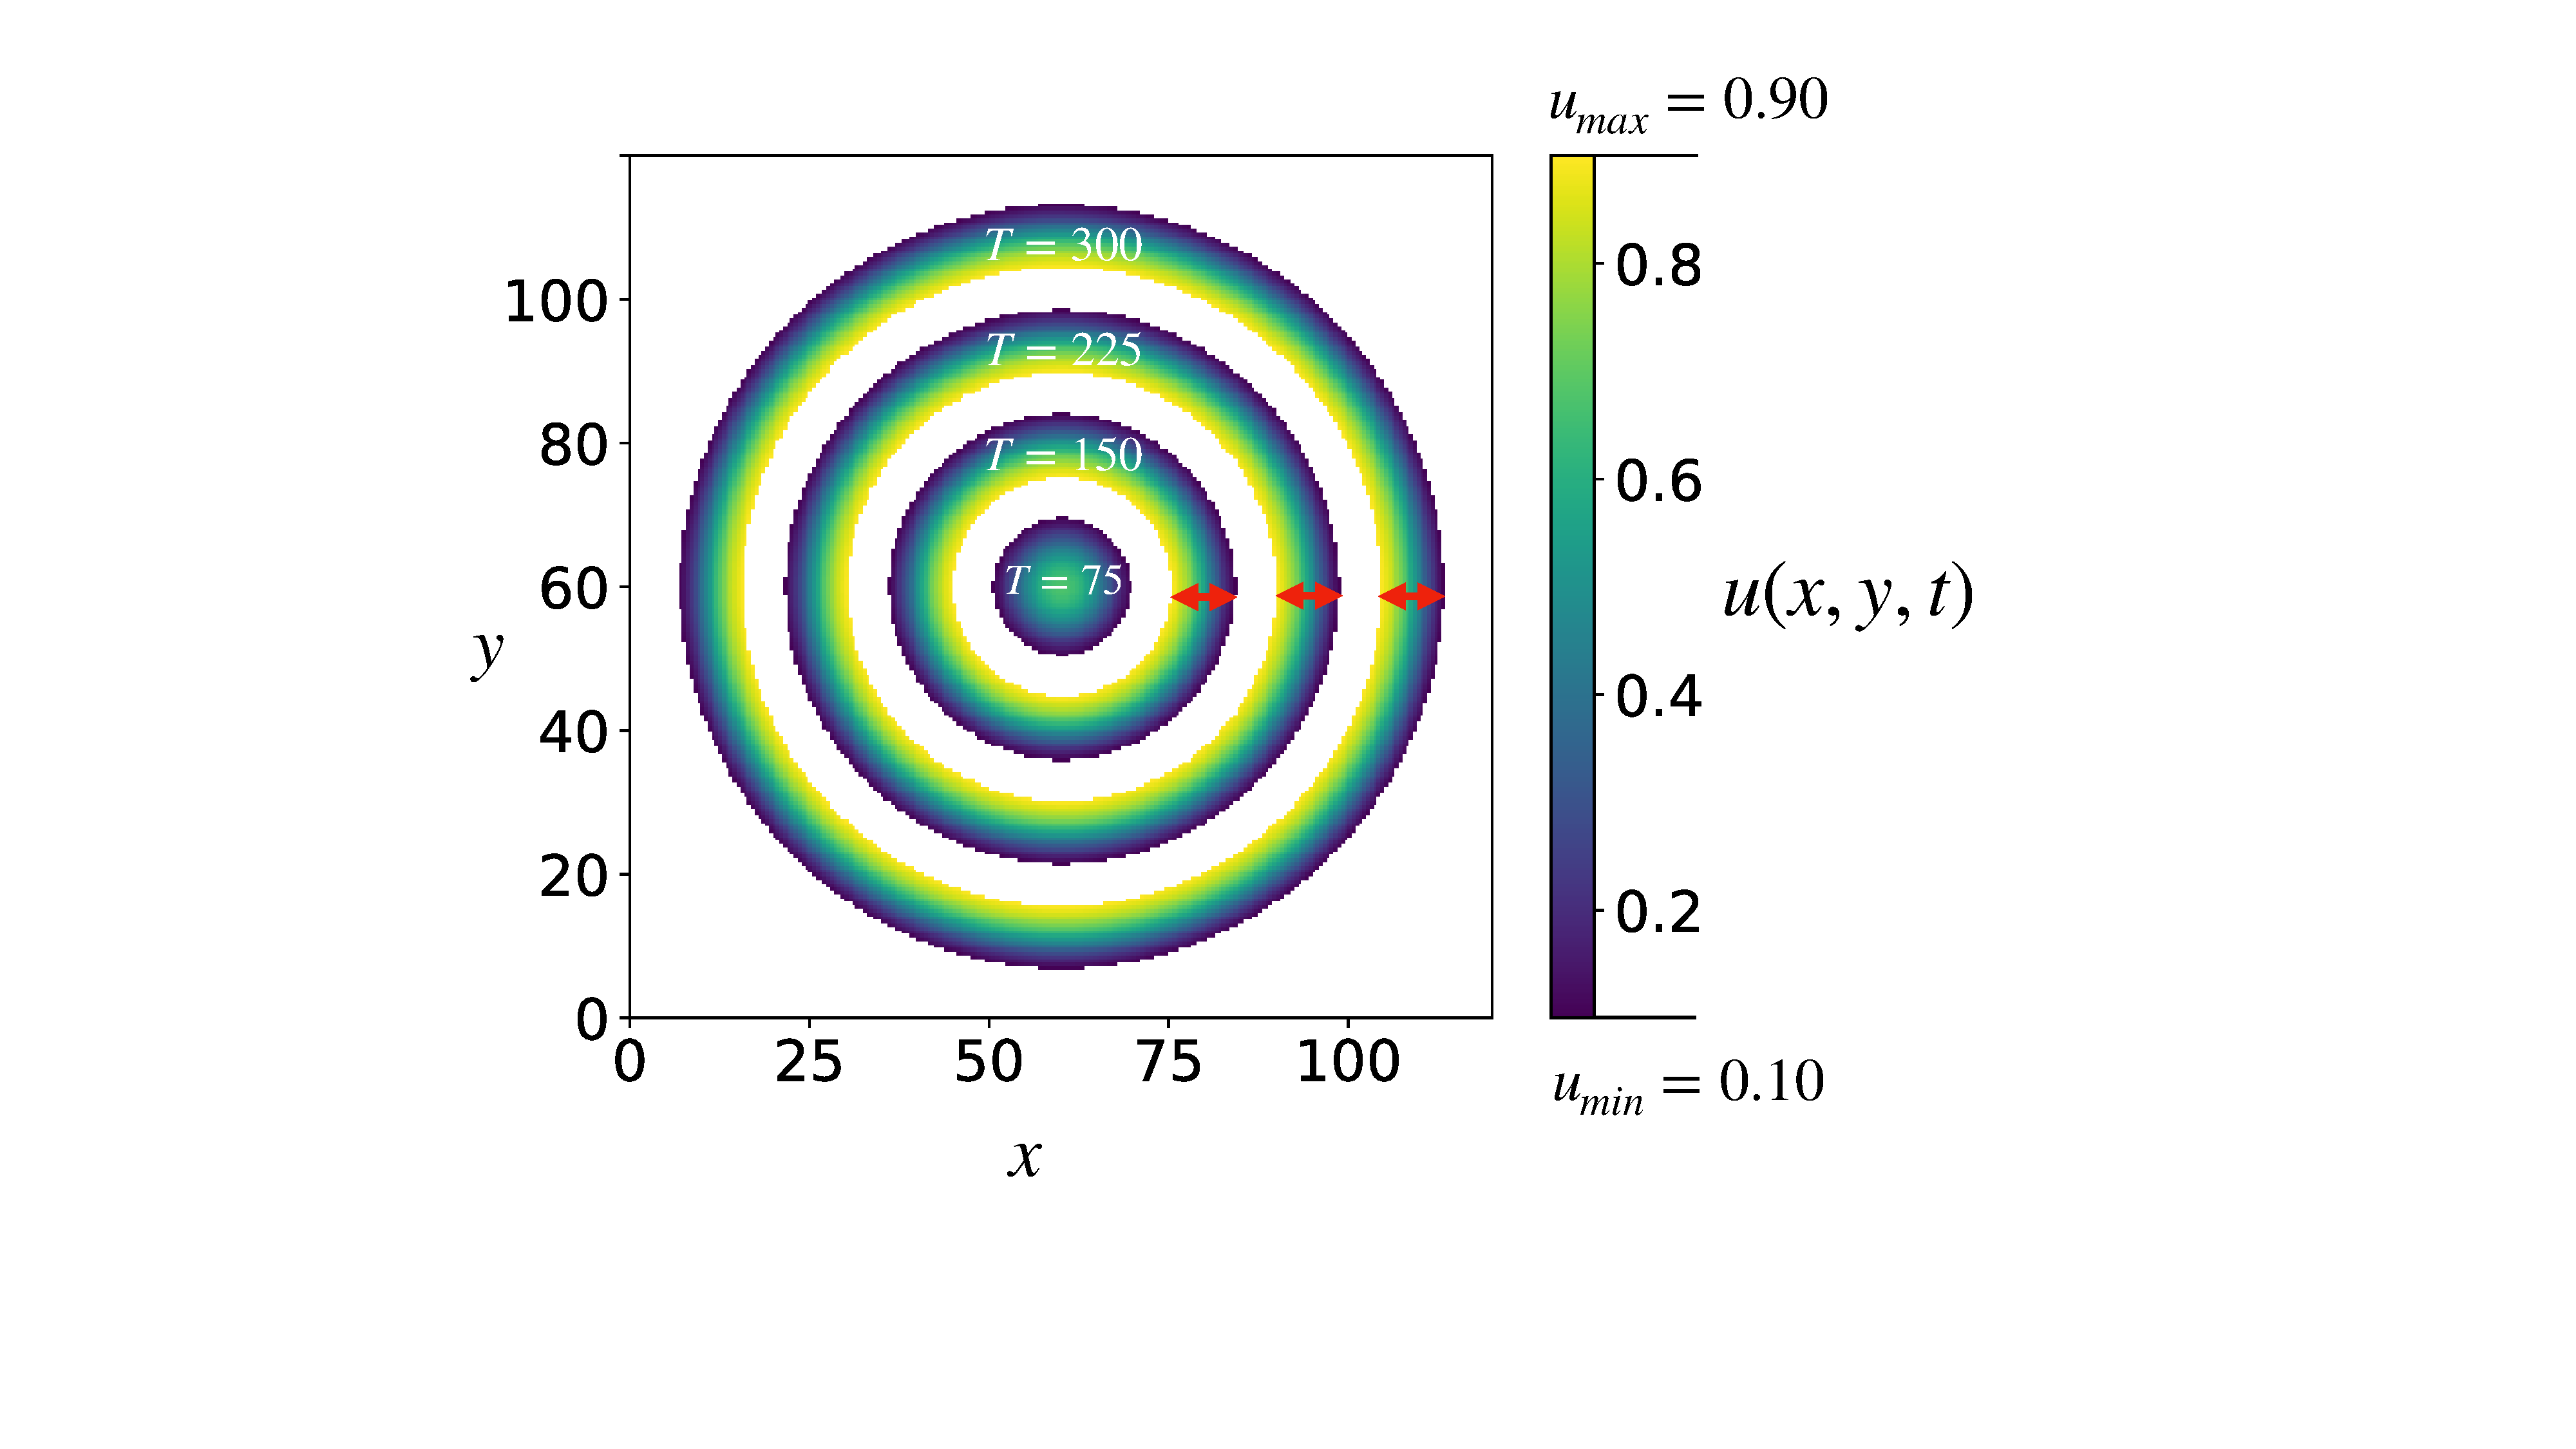
\includegraphics[scale=0.25]{chapter7/figures/figure2x.pdf}
    \caption{A simulation of the FKPP model wave-front for $r=0.10$ and $\mathcal{D}=0.10$ in two spatial dimensions. A non-zero field value is initialised at the domain center at time $t=0$. The field values $0.10 < u < 0.90$ are used to trace out the evolving wave-front and ascertain the speed of propagation. Uniform growth and diffusion give rise to a symmetric front that propagates with constant speed $v=0.200$.}
    \label{fig:fkpp-expo2D}
\end{figure}

Figure \ref{fig:fkpp-expo1D} shows the simulated FKPP model in one spatial dimensions using a forward-time centred-difference (FTCD) scheme, see Appendix \ref{a:pde}. Constant diffusion and growth coefficients, $r=0.05$ and $\mathcal{D}=0.10$, lead to a travelling wave that propagates in the positive $x$ direction with constant speed. The travelling wave solutions of Eq \ref{eq:fkpp-expo} can be shown to advance with speed:
\begin{equation}
    \label{eq:fkpp_vel}
    v \geq v_{min} = 2\sqrt{r\mathcal{D}}
\end{equation}
where $v_{min}$ is the minimum wave-speed admitted by the front, see \cite{murray1993mathematical} for a complete derivation. %
For the purpose of modelling an epidemiological wave, it suffices to take $v\approx v_{min}$ as an approximation to the speed of propagation. %
Using Eq \ref{eq:fkpp_vel} the predicted wave-front speed in Figure \ref{fig:fkpp-expo1D} is given by $v=0.200$. %
The numerical stability of simulations is ensured provided that the Courant–Friedrichs–Lewy (CFL) condition is met\cite{cfl-condition}. %
In the case of the FKPP model, the CFL condition is given by:
\begin{equation}
    \mathcal{D} \frac{dt}{dx^2} < \frac{1}{2}
\end{equation}
where $dx$ and $dt$ represent the discretized domain and time-steps respectively. %
The observed wave-speed of simulations can be calculated by %
tracing the time-evolution of the wave-front mid-point (ie. where $u(x) = \frac{1}{2}$). %
After initial transience, the wave-front in Figure  \ref{fig:fkpp-expo1D} was found to evolve with speed $0.199$ with discretized steps $dx=0.50$ and $dt=0.10$. %

The two dimensional variant of the FKPP model is similarly given by:
\begin{equation}
    \frac{\partial u}{\partial t} = \mathcal{D}\nabla u + ru(1 - u)
\end{equation}
where the field $u$ is now a function of both $x$ and $y$. %
Strictly speaking, Eq \ref{eq:fkpp_vel} is only valid for a one dimensional domain, however, it was found to offer a close approximation for the two dimensional wave-speed,  \textcolor{red}{SEE APPENDIX \ref{a:pde}}. %
\textcolor{red}{Murray, find that curvature 1/r approximation, eq 6.2 only valid for a straight front}. %
Using a FTCD scheme with steps $dx = 0.50$ and $dt = 0.10$, the measured front-speed of the field $u$ in Figure \ref{fig:fkpp-expo2D} was found to be $v=0.189$. %
Using smaller discretized steps of $dx = 0.25$ and $dt = 0.05$ the front-speed can be improved to $v=0.200$ to three decimal places.

Crucially, $\mathcal{D}$ and $r$ control the thickness of the wave front, shown by the red arrows in Figure \ref{fig:fkpp-expo2D}. %
Approximately, the length-scale of the wave-front $\ell_{w}$ can be informed by the quantity $\sqrt{ \frac{\mathcal{D}}{r}}$ (as can be seen by the cancellation of units $\frac{length^2}{t} \frac{1}{t^{-1}}$). %
This can have useful epidemiological implication and is  discussed later on. 

\section{FKPP\textemdash coupling to non-local dispersal model}

The travelling wave solutions of the FKPP model presents a simple starting place to model the spread of disease through a population of trees. %
However, problems arise when estimating the parameter values of $\mathcal{D}$ and $r$ for a particular pathogen (\textcolor{red}{look into lg Plank-formulation and parameter estimates.}). %
A step toward to overcom this problem % what problem?
can be taken by looking towards the non-local dispersal model established in Chapter \ref{chapter:regional-containment1}. %
Specifically, the FKPP model can be informed by the non-local dispersal model via Eq (\ref{eq:fkpp_vel}).

Given fixed growth rates, the non-local dispersal model can be used to inform diffusion coefficients for the FKPP model. %
Re-arranging Eq (\ref{eq:fkpp_vel}) for the diffusion coefficients leads to $\mathcal{D} = \frac{v^2}{4r}$ and the %
investigation moves toward ascertaining $v$ from the non-local dispersal model. %
Figure \ref{fig:fkpp-sgm-vel} shows the process of informing diffusion coefficients based on simulations of the non-local dispersal model. 

The Gaussian dispersal model defined in Chapter \ref{chapter:regional-containment1} gives rise to an epidemic wave-front, defining an interface between infected and susceptible trees. %
Figure \ref{fig:fkpp-sgm-vel}(a) depicts such an epidemic wave propagating through a domain of size $2\mathrm{km}^2$ for arbitrary parameters shown. 5
A distance can be calculated by assessing the furthest distance of an infected tree away from the epicenter, at the domain center, in this example shown by the blue arrow. %

Recording the maximum distance for each simulation time-step leads to a time-series. %
Figure \ref{fig:fkpp-sgm-vel}(b) shows the time-series generated for fixed parameters $\ell, \beta$ and five values of $\rho$. %
The vertical dashed lines indicate positions in time where the pathogen reached the domain boundary, this is analogous to percolation, see Chapter \ref{chapter:regional-containment1}. %
If the pathogen reaches the domain boundary, the  simulation is terminated. %
At the end of the simulations the last recorded distance is divided by the elapsed time, in order to form a naive estimate for the pathogen wave-speed.\footnote{There are many metrics that could be used to trace the evolving front, such as, radially averaged velocity, radially averaged center of mass velocity, median infected distance and average infected distance. However, ensemble-averaged simulations approach the same value and as such the maximum distance was chosen for simplicity.} %

As discussed in Chapter \ref{chapter:regional-containment1}, a pathogen with parameters below the threshold can spread for a time before becoming extinct. This leads to a non-zero spreading speed being registered even though parameters are below the threshold for propagation. %
If non-zero wave-speeds are registered, inferred diffusion coefficients would also assume non-zero values and given the FKPP model levels of infection would logistically increase to unity. %
This is clearly unrealistic for parameters below the threshold for propagation and presents a issue that needs to be addressed and  resolved by considering the wave-speed \textit{multiplied by} the probability of percolation, shown in Figure \ref{fig:fkpp-sgm-vel}. %  

Given stochasticity in the time-series, more reliable estimates for the wave-speed can be generated by ensemble averaging simulations. %
Figure \ref{fig:fkpp-sgm-vel} shows ensemble-averaged results of wave-speed over the parameter space of tree density $\rho$ and pathogen infectivity $\beta$. %
Solid lines show the ensemble-averaged wave-speeds corrected for by multiplying by the probability of percolation. %
Dashed lines show only the wave-speed, without multiplying by the probability of percolation. Dashed lines emphasize regions of parameter space that would be subject to pathogen extinction, pinning these regions to zero keeps the generated diffusion coefficients to zero and constrains spreading in the FKPP model.

Figure \ref{fig:fkpp-sgm-vel}(c) and Eq (\ref{eq:fkpp_vel}) present a mapping function to FKPP diffusion coefficients. %
This relies on fixed growth rates, $r$, and informed tree densities $\rho$. %
As in Chapter \ref{chapter:regional-containment1}, we can use the data-sets reported by \cite{hill.data} to inform tree canopy cover and values of $\rho$ (tree density) over Great Britain. %

Figure \ref{fig:fkpp-diff}(a) shows the diffusion coefficients generated for fixed values $r=0.01\ \mathrm{day^{-1}},\ \beta=0.020\ \mathrm{day^{-1}},\ \ell=25\ \mathrm{m}$ projected onto the Ash tree abundance data from \cite{hill.data}. %
First, each pixel of tree density is mapped onto a predicted wave-speed using results from the non-local dispersal model shown in Figure \ref{fig:fkpp-sgm-vel}(c). %
Each pixel-valued wave-speed is then mapped to a diffusion coefficient using Eq(\ref{eq:fkpp_vel}). %
This paradigm constitutes a continuum-based variant of the sub-grid model presented in Chapter \ref{chapter:regional-containment1}. %
This time however, the model does describe dynamic spread of the pathogen. 

A zoomed $150\mathrm{km^2}$ subset of the diffusion coefficients is plotted in the inset. %
Figures \ref{fig:fkpp-diff}(b-d) depict the FKPP model running with the sub-grid informed diffusion coefficients and a fixed value of $r=0.01\ \mathrm{day^{-1}}$ from years $1, 5, 10$ respectively. %
Initially, a small patch of land $5\mathrm{km^2}$ is infected with a value of $u=0.10$ pathogen occupation. Growth and spread of the pathogen can then be seen to take place in the form of a wave-front.  %

As the field $u$ is bounded between $[0, 1]$, fixing the growth rate to $r=0.01\ \mathrm{day^{-1}}$ approximates a reasonable, %
albeit uninformed, growth rate of a pathogen\footnote{For a fixed growth rate of $r=0.01$, it takes approximately $2$ years for an initially infected field value of $u(x)=0.01$ to attain a final value of $u(x)=0.95$ pathogen occupation.}. %
The final extent of pathogen spread over a $10$ year period is indicated by the double arrow in Figure \ref{fig:fkpp-diff}(d) spanning a distance of $\sim 35\mathrm{km}$. %
From this, we can see that the spreading rate is too small in comparison to a typical epidemic (see \cite{dutch-elm-mismanage} for a discussion on the Dutch elm disease epidemic) and presents a set of problems with the model. %


\begin{figure}
    \centering
    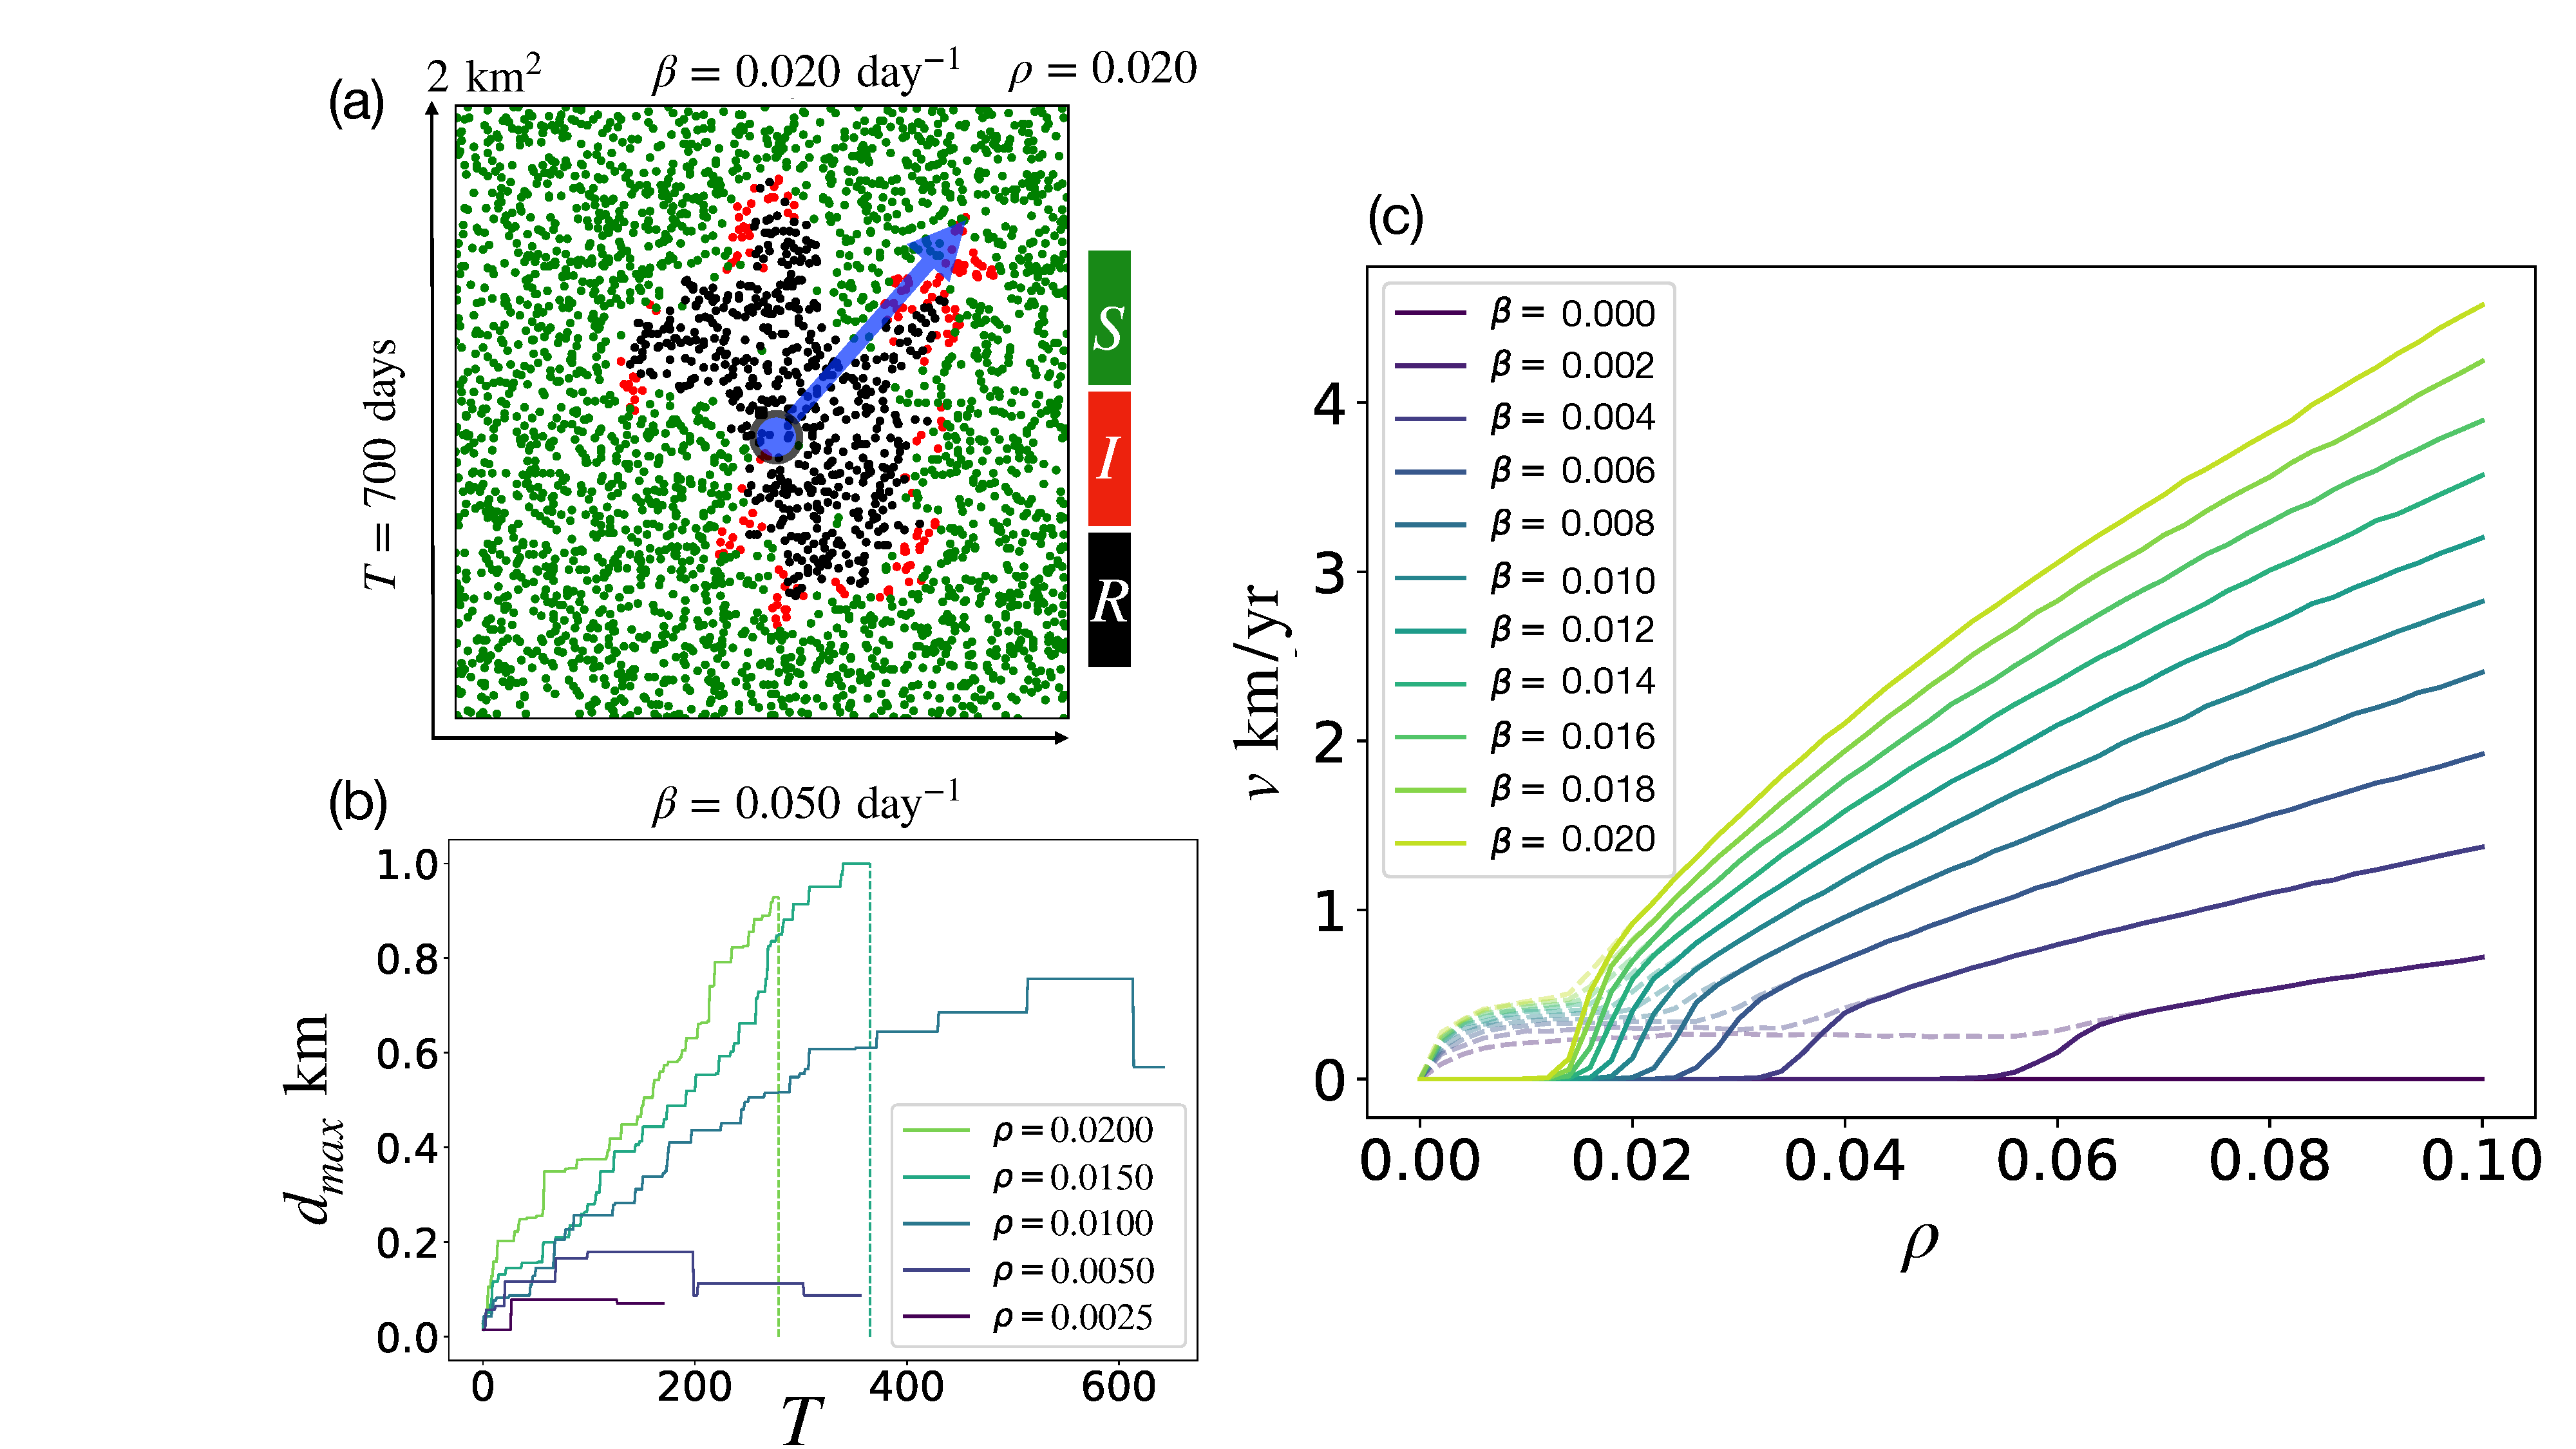
\includegraphics[scale=0.25]{chapter7/figures/figure3x.pdf}
    \caption{Generating estimates of the epidemic wave-speed from the non-local dispersal model, for fixed dispersal distance $\ell = 25\ \mathrm{m}$. (a) For each time-step in the dispersal model, a distance can be calculated by assessing the furthest position of an infected/removed tree away from the epicenter. (b) The time-series of maximum-distance is shown for fixed infectivity $\beta$ and five different parameter values of density $\rho$. An estimate for wave-speed is formed by dividing the maximum-distanced reached by the total elapsed time of the simulation. (c) Ensemble-averages of the wave-speed are shown for different combinations of $\rho$ and $\beta$.}
    \label{fig:fkpp-sgm-vel}
\end{figure}

\begin{figure}
    \centering
    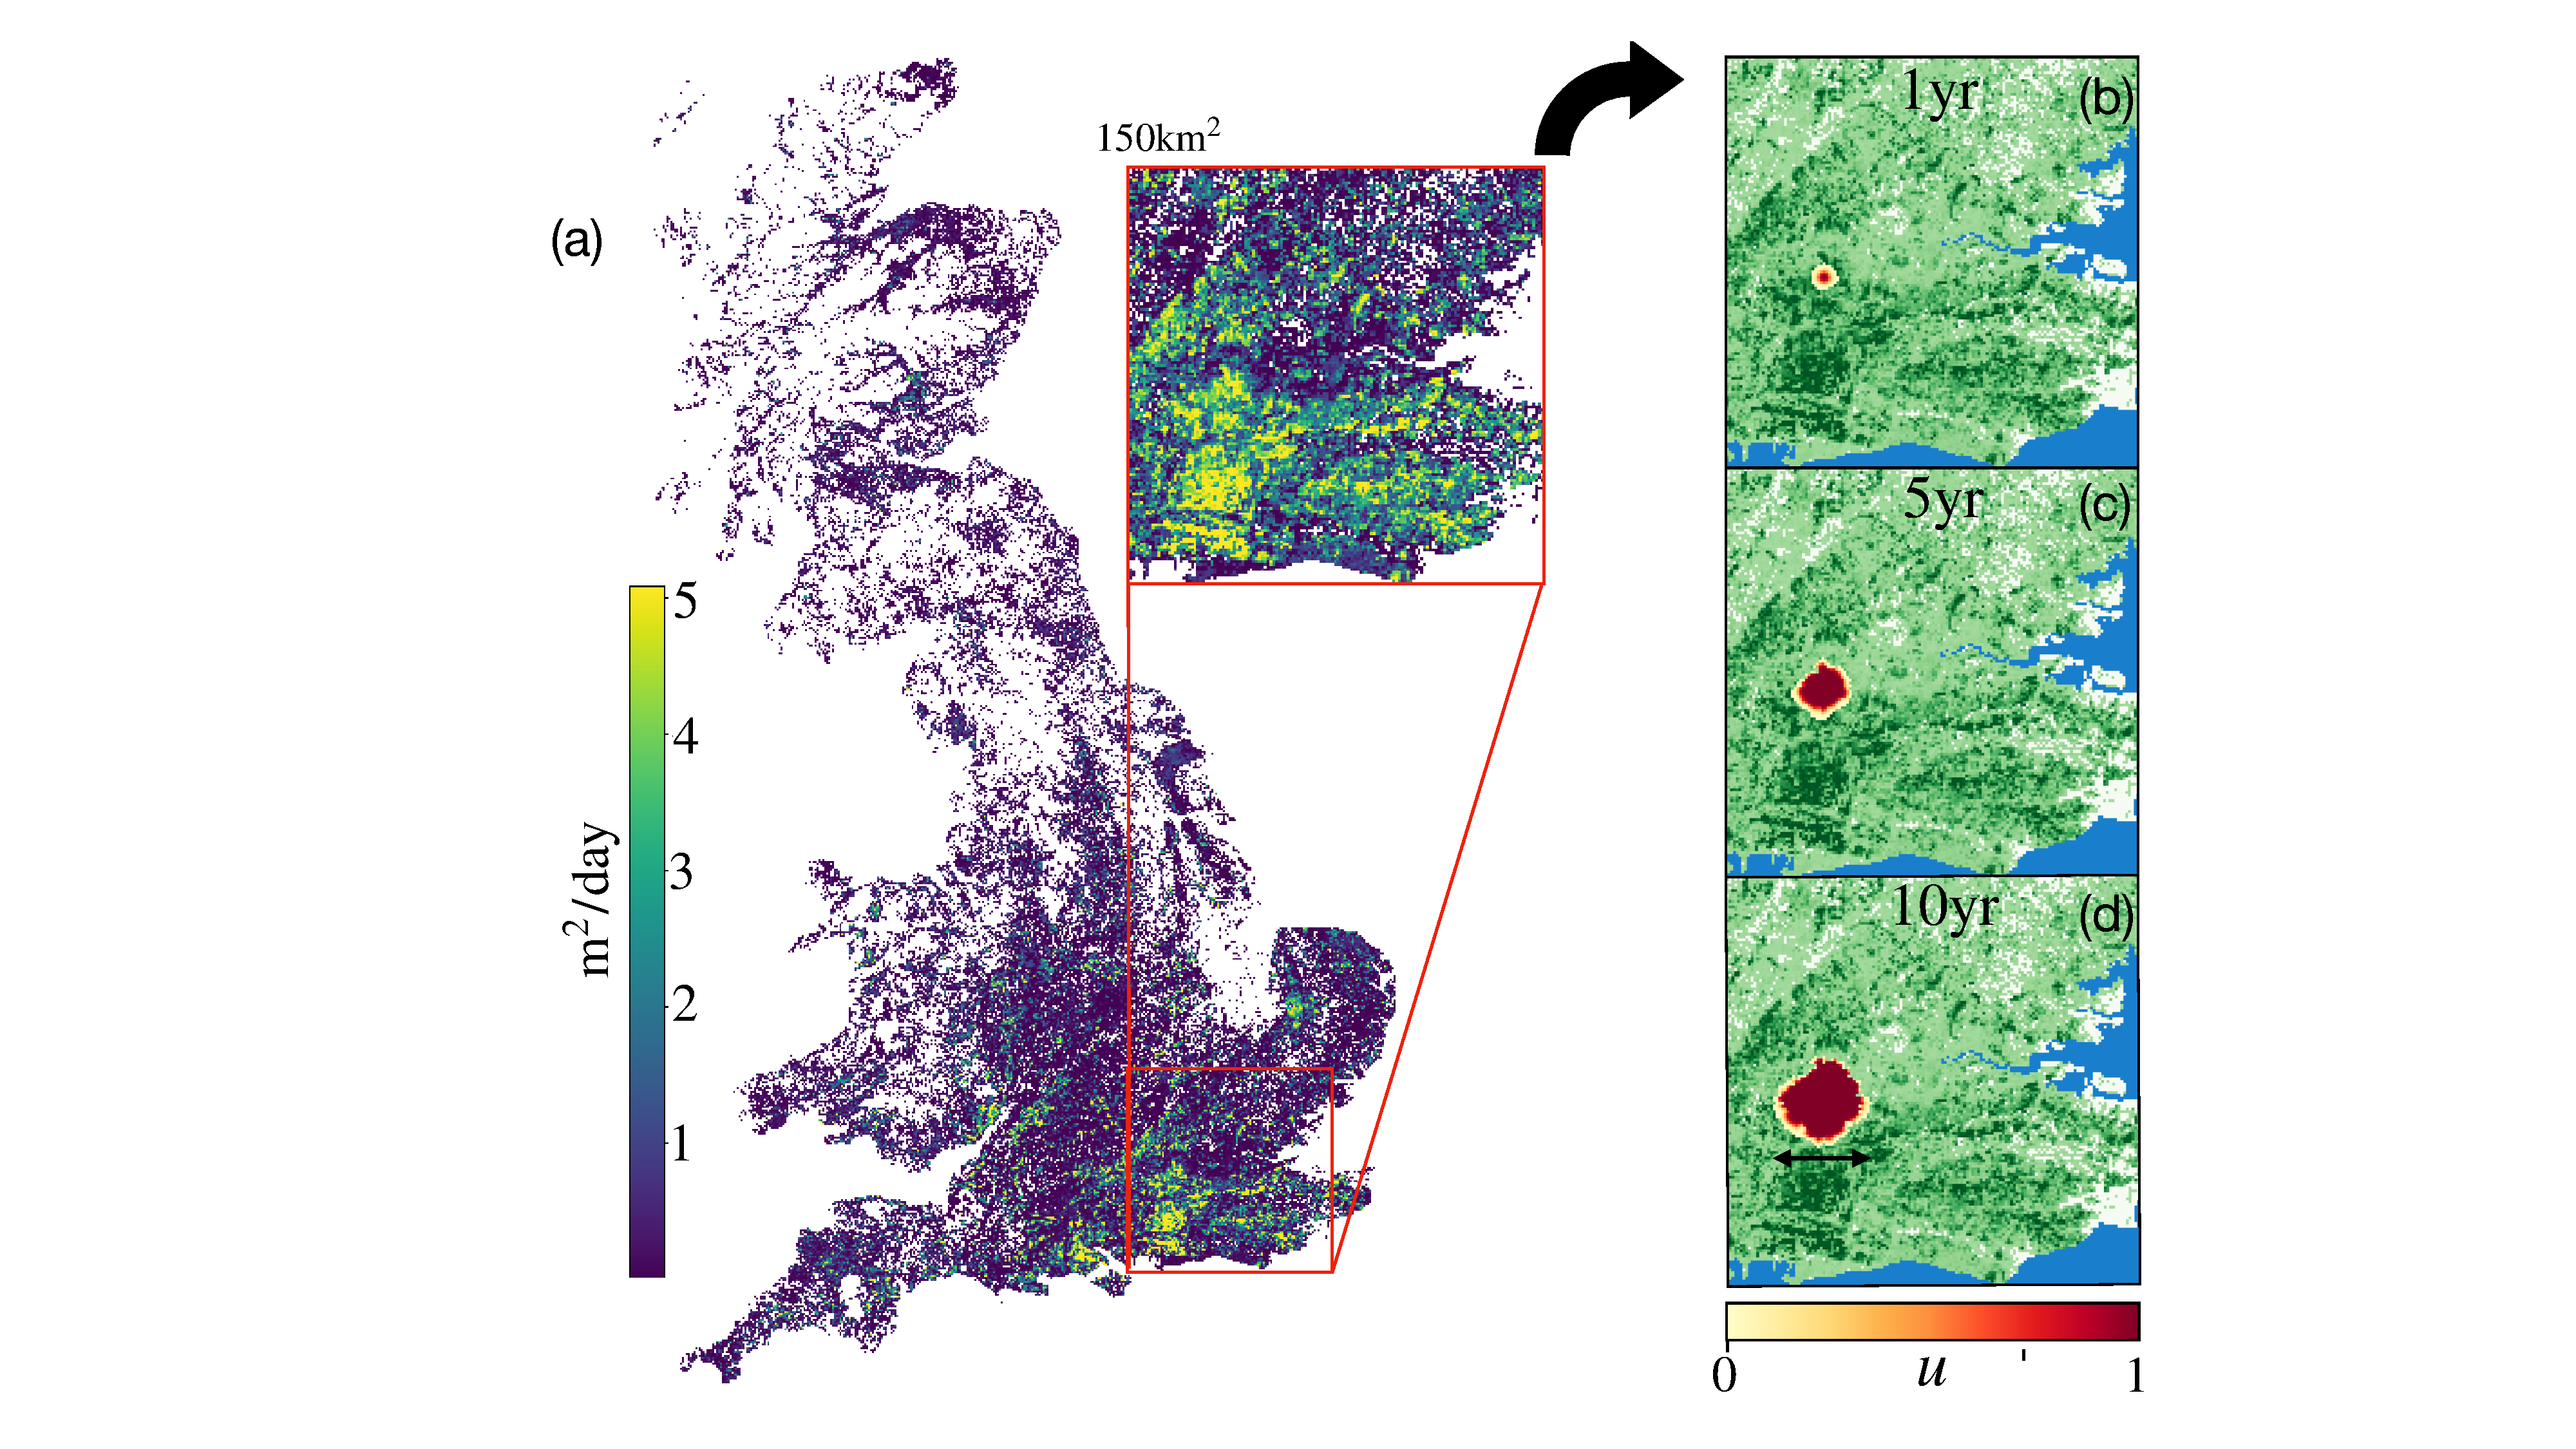
\includegraphics[scale=0.30]{chapter7/figures/figure4x.pdf}
    \caption{Diffusion coefficients generated from the sub-grid dispersal model for fixed parameters $r=0.01\ \mathrm{day^{-1}},\ \beta=0.020\ \mathrm{day^{-1}},\ \ell=25\ \mathrm{m}$. Diffusion value are projected onto the canopy cover data for Great British Ash distribution reported by \cite{hill.data}.}
    \label{fig:fkpp-diff}
\end{figure}

In the model,  constructed so far, there are three parameters that control the rate of spread: $\rho$, $\beta$ and $\ell$. %
Given that $\rho$ is fixed by the number of trees in the system, the only way to increase the speed of spread is to increase $\beta$ or $\ell$ (or both). %
However, as shown in Chapter \ref{chapter:regional-containment1} the relationship between $\beta$ and $\ell$ can be approximated to follow $\beta \propto \ell^{-2}$. %
Therefore, in order for the pathogen to spread faster the infectivity rate must substantially decrease in order to constrain realistic values of $R_0$. This precludes the possibility of increasing both $\beta$ and $\ell$ simultaneously. %

In order to avoid modelling unrealistic values of $R_0$ whilst increasing the rate of spread, %
we are left with the two options of increasing $\beta$ and decreasing $\ell$, or vice versa. %
Consider the thought experiment of increasing $\beta$ and decreasing $\ell$. Doing so would lead to more secondary infections inside a smaller area set by the dispersal kernel. %
On the other hand, if $\ell$ is increased and $\beta$ decreased, more secondary infections would result at further distances away from the infectious source. %
Thus, increasing $\ell$ and decreasing $\beta$ would at first appear to be means of constraining $R_0$ and increasing the speeds shown in Figure \ref{fig:fkpp-sgm-vel}(c). %
However, this in-turn leads to a problem which calls into question the validity of Gaussian dispersal. %


When $\ell$ becomes large in comparison to the average space between trees, %
a lower-rate of secondary infections amongst nearest-neighbours is observed in comparison to trees further away. %
This results because close to the source of infection, the  Gaussian dispersal does not decay rapidly enough. Pathogen dispersal with high values of $\ell$ can therefore become insensitive to immediate neighbours leading to a loss of short-range structure in the model. %
This exists in stark contrast to the intuitive notion that nearest-neighbours will become infected first, in response to an infected source. %
As discussed in Chapter \ref{chapter:regional-containment1} Gaussian dispersal was merely chosen as a convenient approximation. The limits of this approximation are now clearly exposed in the face of modelling longer-range dispersal events. %

%finish this please 
\section{Exponential dispersal}
%finish this please 
In Chapter \ref{chapter:regional-containment1}, the reproductive number $R_0$ of the model was explored in detail. Parameter values of $\beta=0.005\mathrm{day^{-1}}$ and $\ell\mathrm{m}$ were considered based on constraints of $R_0$, that is, roughly speaking $R_0 \in [0, 10]$. 
%finish this please 
\blindtext[1]
\blindtext[1]




\section{Chapter summary}
%finish this please 
\blindtext[1]
\textcolor{blue}{Detail all... the above...}




